\documentclass[UTF8, twocolumn ]{ctexart}
\usepackage{graphicx}
\usepackage{amsmath}
\usepackage{paralist}
\usepackage[
  colorlinks,
  linkcolor = black
]{hyperref}

\usepackage{fancyhdr}                                
\usepackage{lastpage}                                           
\usepackage{layout}                                                                          

\linespread{1.56}
\columnsep = 15pt
\begin{document}

\title{\huge{基于正态分布概率计算和支持向量机计算的WIFI定位技术}}
\author{北京优锐科技有限公司\ 丁贵金\ 朱韬\ 袁万尚}
\date{\today\\*\ \hrule}
\maketitle

%%%%%%%%%%%%%%%%%%%%%%%%%%%%%%%%%%%%%%%%%%%%%%%%%%%

\begin{abstract}
基于正态分布概率和支持向量机原理的WIFI定位技术,完全采用软件通过科学计算来实现。该技术不需要依赖专用设备,部署简单使用便捷,对环境无强制依赖,可以在复杂WIFI环境下实现移动设备精确定位。该WIFI定位技术的核心原理是支持向量机,辅助计算的数学工具是正态分布的概率模型。整体技术框架为,采用正态分布概率模型筛选校准信息,同时确定移动设备大致方位,之后将筛选出的校准信息与移动设备实时采集到的WIFI信息进行支持向量机计算,最终确定移动设备的准确位置。该技术不依赖特殊硬件设备,不对环境做特殊要求,旨针对实际应用提供完整技术方案。
\par
\noindent{\textbf{关键词}:}
待定位点(LP),校准点(CP),WIFI接入点(AP),标准差($\mathnormal{\sigma}$),方差($\mathnormal{\sigma}^{2}$),正态分布(Normal),支持向量机(SVM),概率(Pl),WIFI信号值(RSS),WIFI信号平均值(mRSS)
\end{abstract}

%%%%%%%%%%%%%%%%%%%%%%%%%%%%%%%%%%%%%%%%%%%%%%%%%%%

\section{引言}
WIFI定位技术目前有多种实现方法,但在具体应用中都存在一些限制和缺陷。
\par
一般的WIFI定位技术对环境要求比较严格,需要在环境中部署固定AP或使用专用硬件设备,一旦这些条件缺失,WIFI定位功能则无法工作。并且使用WIFI定位的移动终端设备也必须符合事先约定的要求,因为不同的移动终端设备,对WIFI信号的接收能力有所不同,无法实现任意设备在任意环境中的WIFI定位。
\par
本文详细说明了采用概率和支持向量机原理实现的WIFI定位技术,目的是依靠纯软件实现移动设备在有限空间内的定位功能,不依赖环境中的特殊AP属性,不用添加专用硬件设备。
\par
本文所阐述的技术原理是纯粹的计算机科学计算,通过数学概率原理实现对环境中AP分布状态的数学模拟,通过支持向量机计算实现对移动终端设备的位置确定。这些数学模型不依赖具体硬件设备,而不同硬件设备的特征作为数学系数可以根据不同设备的特点进行调整。这样的设计,就可以实现不同设备的定位计算过程统一,使本文所阐述的技术适用于任意环境中的任意设备。
\par
本文在阐述WIFI定位技术的过程中,也对技术实现中遇到的具体问题做了充分说明,并提供了具体的解决方法,如环境中AP的变动或意外缺失发生时,对定位过程的影响和解决方法,不同移动终端设备做校准操作时的具体过程和方法,以及对于少数无法定位时的状态处理等。
\par
本文的“原理”部分,主要阐述技术的理论依据和所采用的数学模型,“方法”部分则具体阐述技术实现过程,“结果”部分归纳了该技术的最终应用模式,“技术创新”部分具体说明该技术的先进,与同类技术相比下的优势,“应用前景”部分介绍了该技术实际应用的具体形式,以及对采用该技术的行业所产生的积极作用。

%%%%%%%%%%%%%%%%%%%%%%%%%%%%%%%%%%%%%%%%%%%%%%%%%%%

\section{原理}
本文所阐述的技术原理,主要包括如下两个方面:
\begin{compactitem}
\item\textbf{空间的数学建模原理}
\item\textbf{定位过程的数学计算原理}
\end{compactitem}
\par
主要使用的数学工具是:
\begin{compactitem}
\item\textbf{正态分布概率计算}
\item\textbf{支持向量机计算}
\end{compactitem}

\subsection{利用WIFI设备和信号对有限空间的数学模拟}
在一个有限空间内,任意分布着多个WIFI信号接入设备(AP),这些设备的分布状态和自身信号强弱,形成了一个向量集合。该有限空间内的不同位置,都对应一个唯一的向量,这个唯一向量可以作为该有限空间内这个位置点的数学量化标示。我们在一个有限空间内,划分多个小区域,每个小区域中都找一个位点作为该小区域的位置校准点(CP)。
\par
当一个移动终端设备出现在这个有限空间内的某个位置,它所能搜索到的AP设备数量和每个AP的信号强度,与这个有限空间内的所有CP做概率计算,会得到一组对应于每个CP的数学概率值,这组概率值中最大的两个CP,就能够确定这个移动设备在该空间内小区域的大致方位。
\par
该移动设备在该空间内不同位置上,所接收到的AP设备和这些AP的信号强度都不会雷同,并且移动设备所收集到的AP信息根据自身位置不同而发生线性变化。
\subsection{在有限空间内建立校准点和生成校准表}
在一个有限空间内划分出覆盖整个空间的若干小区域,规定每个区域中的一个位置作为校准点(CP)。通过一个移动终端设备,在每个CP上采样一组AP信息,计算出该CP上有效AP和每个有效AP的信强度平均值。这些AP和每个AP的信号平均值,就可以代表一个CP在这个有限空间内位置的数学期望,而根据信号平均值又可以计算出这个CP上各个AP相对于数学期望的离散程度。将这些数据整理后,就得到了一张对应于该有限空间不同位置的校准数据表。
\subsection{通过正态分布概率计算得到待定位设备所需数据}
当一个移动终端设备出现在该有限空间内时,这个设备所在的位置就是一个待定位点(LP)。该设备在LP上会收集到一组AP的信息,通过将这组AP信息和校准表上各CP中所有AP的离散值进行概率计算,便可以得到这个LP可能出现在每个CP上的概率值,而概率值最大的几个CP便可以确定该设备有可能出现在有限空间内的几个小区域。
\subsection{通过支持向量机计算确定待定位设备的准确位置}
得到了LP的大致方位,就可以采用支持向量机的数学模型来对移动设备进行精确定位。将概率最大的两个CP上有效的AP信息和他们所标示的位置一一对应,再将待定位移动设备上收集到的AP信息与这两组向量做支持向量机计算,并得到一个确定的对应位置,该位置就是这个移动设备出现在该有限空间内的相对准确位置。
\subsection{原理总结}
用概率计算,得到移动设备进行精确定位时所需数据,再用支持向量机计算移动设备的精确位置,可以避免软件进行大量的无效计算,也可以避免无效数据进入支持向量机的计算过程。通过概率计算的筛选,提高了WIFI定位过程的效率,也实现了概率与支持向量机计算的有效结合提高了定位准确性。

%%%%%%%%%%%%%%%%%%%%%%%%%%%%%%%%%%%%%%%%%%%%%%%%%%%

\section{方法}
本文阐述的技术实现方法,涉及到网络通讯、科学计算、数据库相关技术。服务器负责地图、位置信息、校准数据和科学计算等功能。移动设备软件负责收集AP信息、向服务器发送信息和接收服务器返回的位置结果。
\par
总体过程如图\ref{fig:1}
\begin{figure}[!ht]\centering
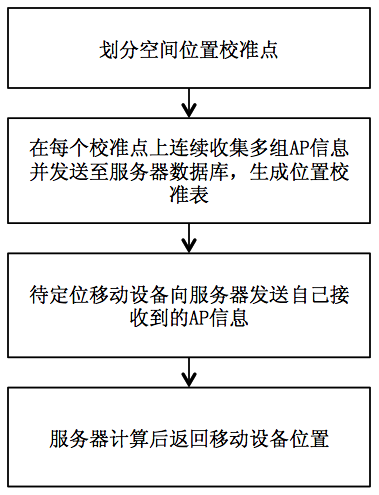
\includegraphics[keepaspectratio, scale=0.45]{no1.png}
\caption{WIFI定位总体过程示意图\label{fig:1}} 
\end{figure}

\subsection{有限空间的位置校准信息采样方法}
第一步,确定一个有限空间的范围,将该空间内划分为多个小区域,每个小区域中确定一个WIFI定位校准点CP。
\par
第二步,用移动设备,在每个CP上采集AP信息,每次采集一组AP数据,同时发送到服务器端,保存至数据库。在同一个CP上,要连续多次采集AP数据,采集次数应该至少不低于5次。
\par
第三步,服务器端将所有CP上收集的AP信息,保存至数据库,将其中信号值为-100的AP信息去除,同时将AP出现次数少于2次的AP信息去除。
\par
第四步,生成WIFI定位原始数据采集表。

\subsubsection{确定空间边界}
这个过程需要根据以下规则执行:
\begin{compactitem}
\item\textbf{确定有效的定位空间}
\item\textbf{确定无效的定位空间}
\item\textbf{有效定空间域和无效定位空间的边界,就是最终定位空间的边界}
\item\textbf{将无效定位空间全部忽略,只记录所有有效定位空间的布局图}
\end{compactitem}
\par
如图\ref{fig:2},图形区域之外的范围都是定位无效空间
\begin{figure}[!ht]\centering
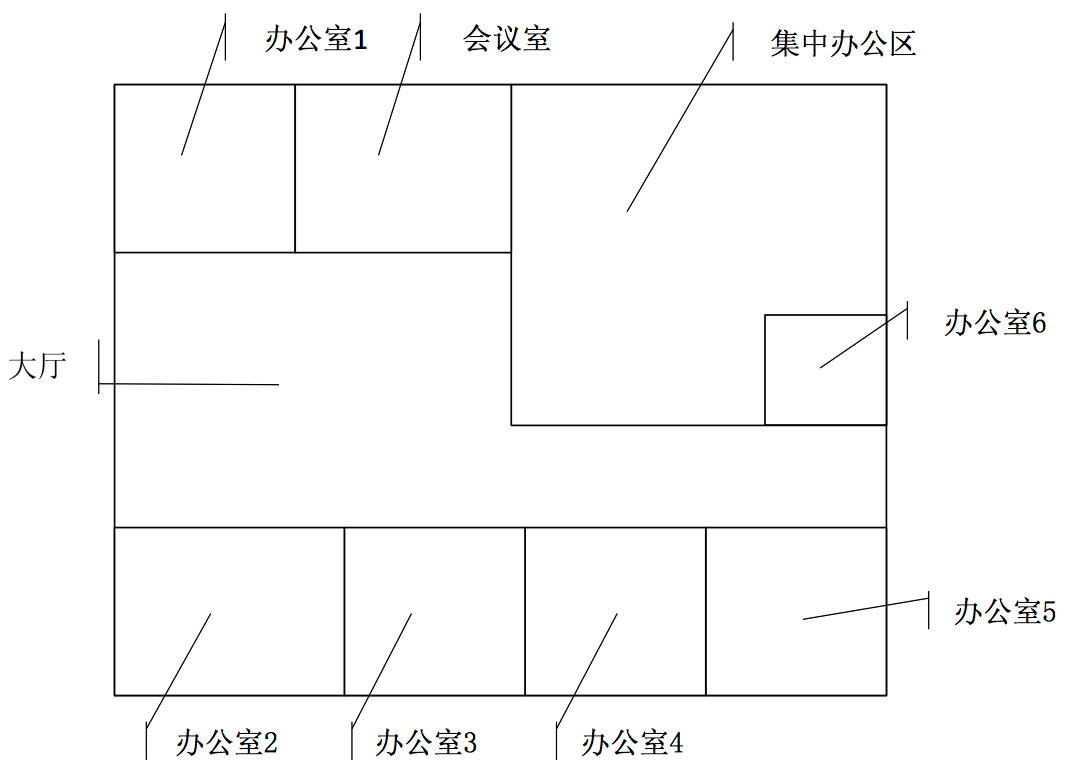
\includegraphics[keepaspectratio, scale=0.2]{no2.png}
\caption{确定空间边界示意图\label{fig:2}} 
\end{figure}

\subsubsection{划分位置区域}
在确定空间边界后,将这个空间根据实际定位需求,划分为多个小区域。实际定位需求,指的就是WIFI定位的目的,必须根据实际空间的状态来划分。通常做法是将空间内的有效使用空间划分为小区域,比如确定一层写字楼为一个需要定位的空间,那么根据实际应用需求,可以将每个办公室或大房间中的每个工作区,划分为小区域。示例如图\ref{fig:3}
\begin{figure}[!ht]\centering
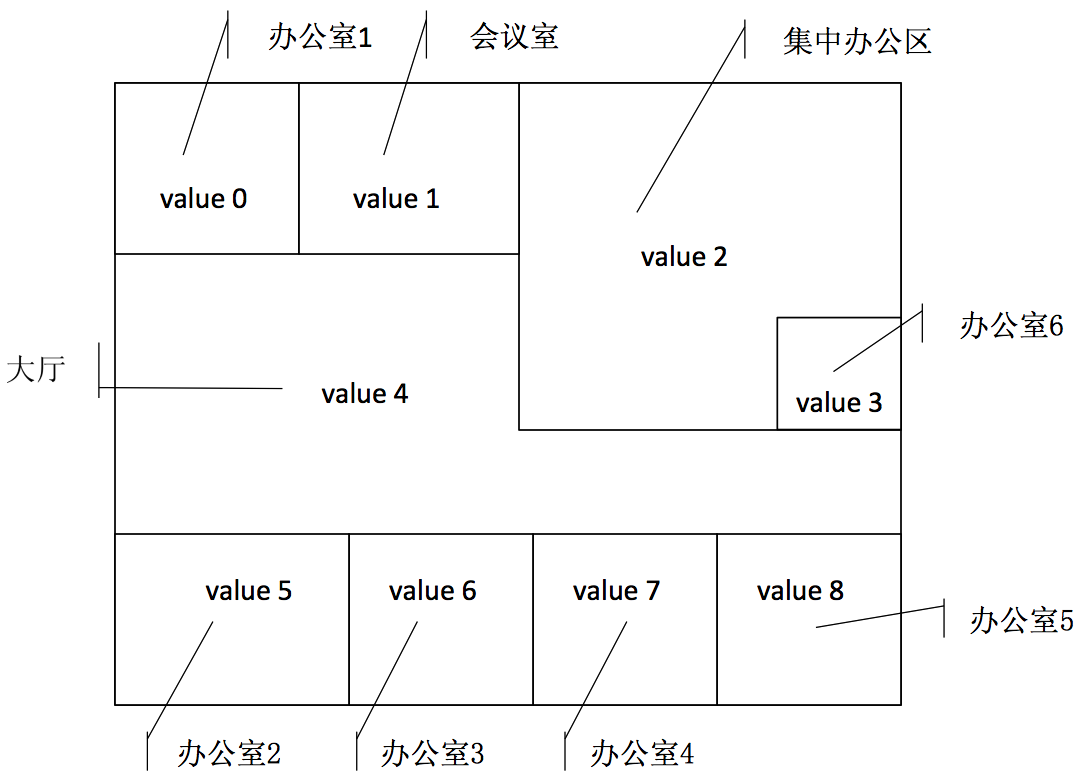
\includegraphics[keepaspectratio, scale=0.2]{no3.png}
\caption{划分位置区域示意图\label{fig:3}} 
\end{figure}

\subsubsection{确定每个区域中的位置校准点CP}
在划分好的小区域中,选择该区域的相对空间中心点,作为WIFI定位校准点CP。示例如图\ref{fig:4}
\begin{figure}[!ht]\centering
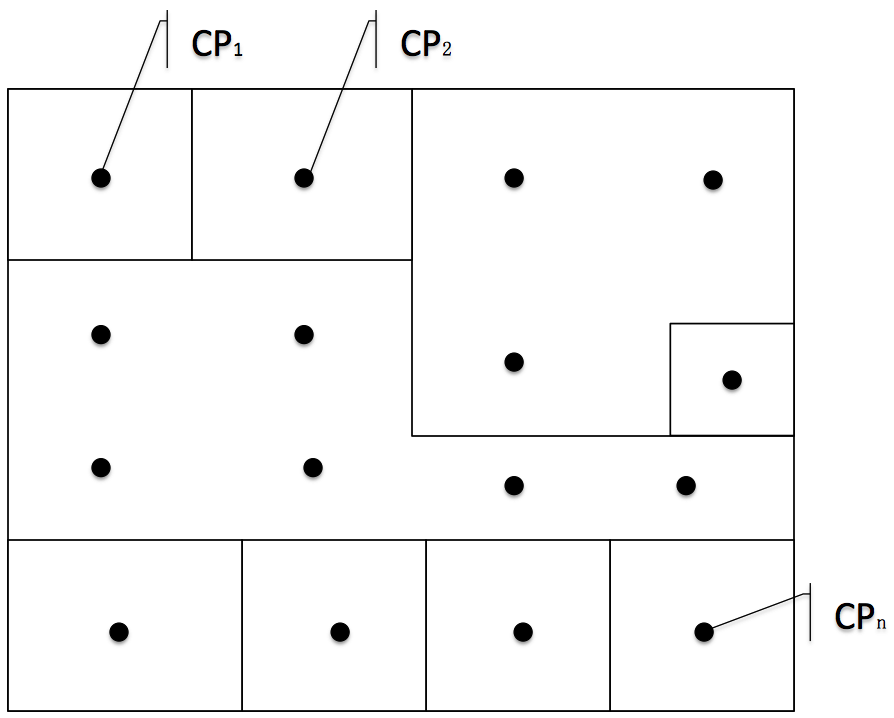
\includegraphics[keepaspectratio, scale=0.2]{no4.png}
\caption{确定位置校准点示意图\label{fig:4}} 
\end{figure}

\subsubsection{在每个CP上采集多组AP信息}
用一台移动终端设备,在每个CP上采集AP信息。每次采集会得到一组AP数据,其中有效数据,是每个AP的MAC地址和每个AP的信号值,为了之后处理数据,还必须同时保存采集数据的时间点,每次采集的一组AP,和采集时间点一一对应,发送至数据库保存。数据库中的最终数据如图\ref{fig:5}:
\begin{figure}[!ht]\centering
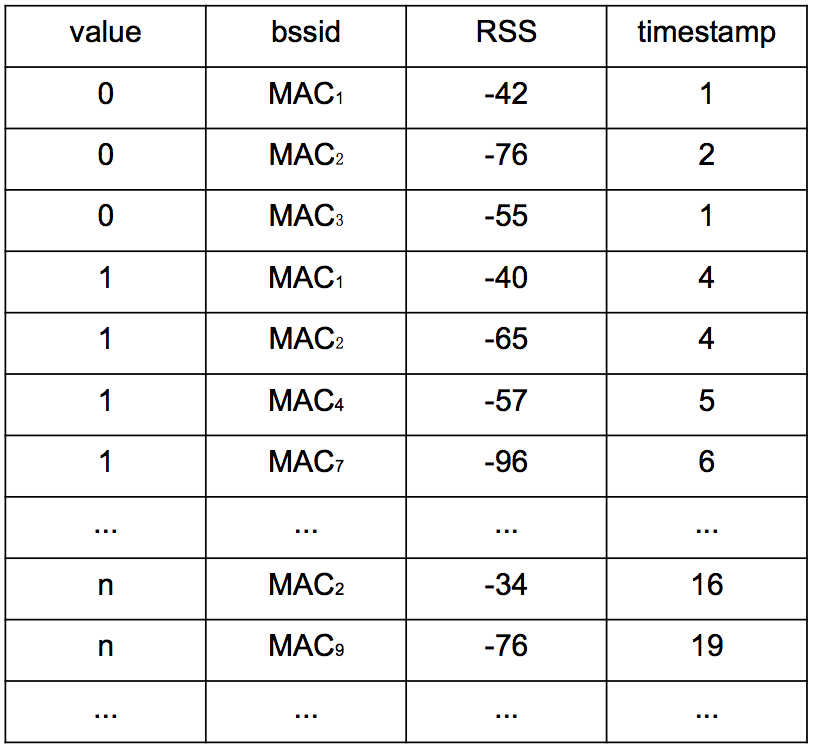
\includegraphics[keepaspectratio, scale=0.26]{no5.png}
\caption{最终定位原始数据表示意图\label{fig:5}} 
\end{figure}
\begin{compactitem}
\item\textbf{value}:定位区域ID
\item\textbf{bssid}:AP的MAC地址
\item\textbf{RSS}:AP的信号值
\item\textbf{timestamp}:采样时间点
\end{compactitem}

\subsection{建立位置校准表}
\subsubsection{计算AP信号物理值}
\subsubsection{计算CP中所有AP信号平均值和标准差}
\subsubsection{生成校准表}

\subsection{LP的信息处理}
完成定位校准表之后,当一个待定位移动设备出现在有效定位空间内,该设备所处的位置,就是一个待定位点(LP),在该LP上会实时接收到一组AP信息,将这组AP信息发送到服务器端,服务器就根据校准表,对LP接收到的AP信息做正态概率计算,最后筛选出两个概率最大的CP信息。
\par
将筛选出的CP数据,和LP发送来的AP数据,做支持向量机计算,得到一个向量集对应的位置ID,该ID就是LP在有效定位空间内的具体位置。
\subsubsection{通过正态分布概率计算筛选有效CP}
\begin{displaymath}
Pl=\frac{1}{\sqrt{2\pi}\sigma}e^{\frac{-(RSS-mRSS)^{2}}{2\sigma^{2}}}
\end{displaymath}

\subsubsection{通过支持向量机计算LP在空间内的位置}

%%%%%%%%%%%%%%%%%%%%%%%%%%%%%%%%%%%%%%%%%%%%%%%%%%%

\section{结果}

%%%%%%%%%%%%%%%%%%%%%%%%%%%%%%%%%%%%%%%%%%%%%%%%%%%

\section{技术创新}

%%%%%%%%%%%%%%%%%%%%%%%%%%%%%%%%%%%%%%%%%%%%%%%%%%%

\section{应用前景}

%%%%%%%%%%%%%%%%%%%%%%%%%%%%%%%%%%%%%%%%%%%%%%%%%%%

\end{document}
